\documentclass{standalone}
\usepackage{tikz}
\usetikzlibrary{patterns, positioning}
\usepackage[sfdefault]{ClearSans} %% option 'sfdefault' activates Clear Sans as the default text font
\usepackage[T1]{fontenc}

\begin{document}
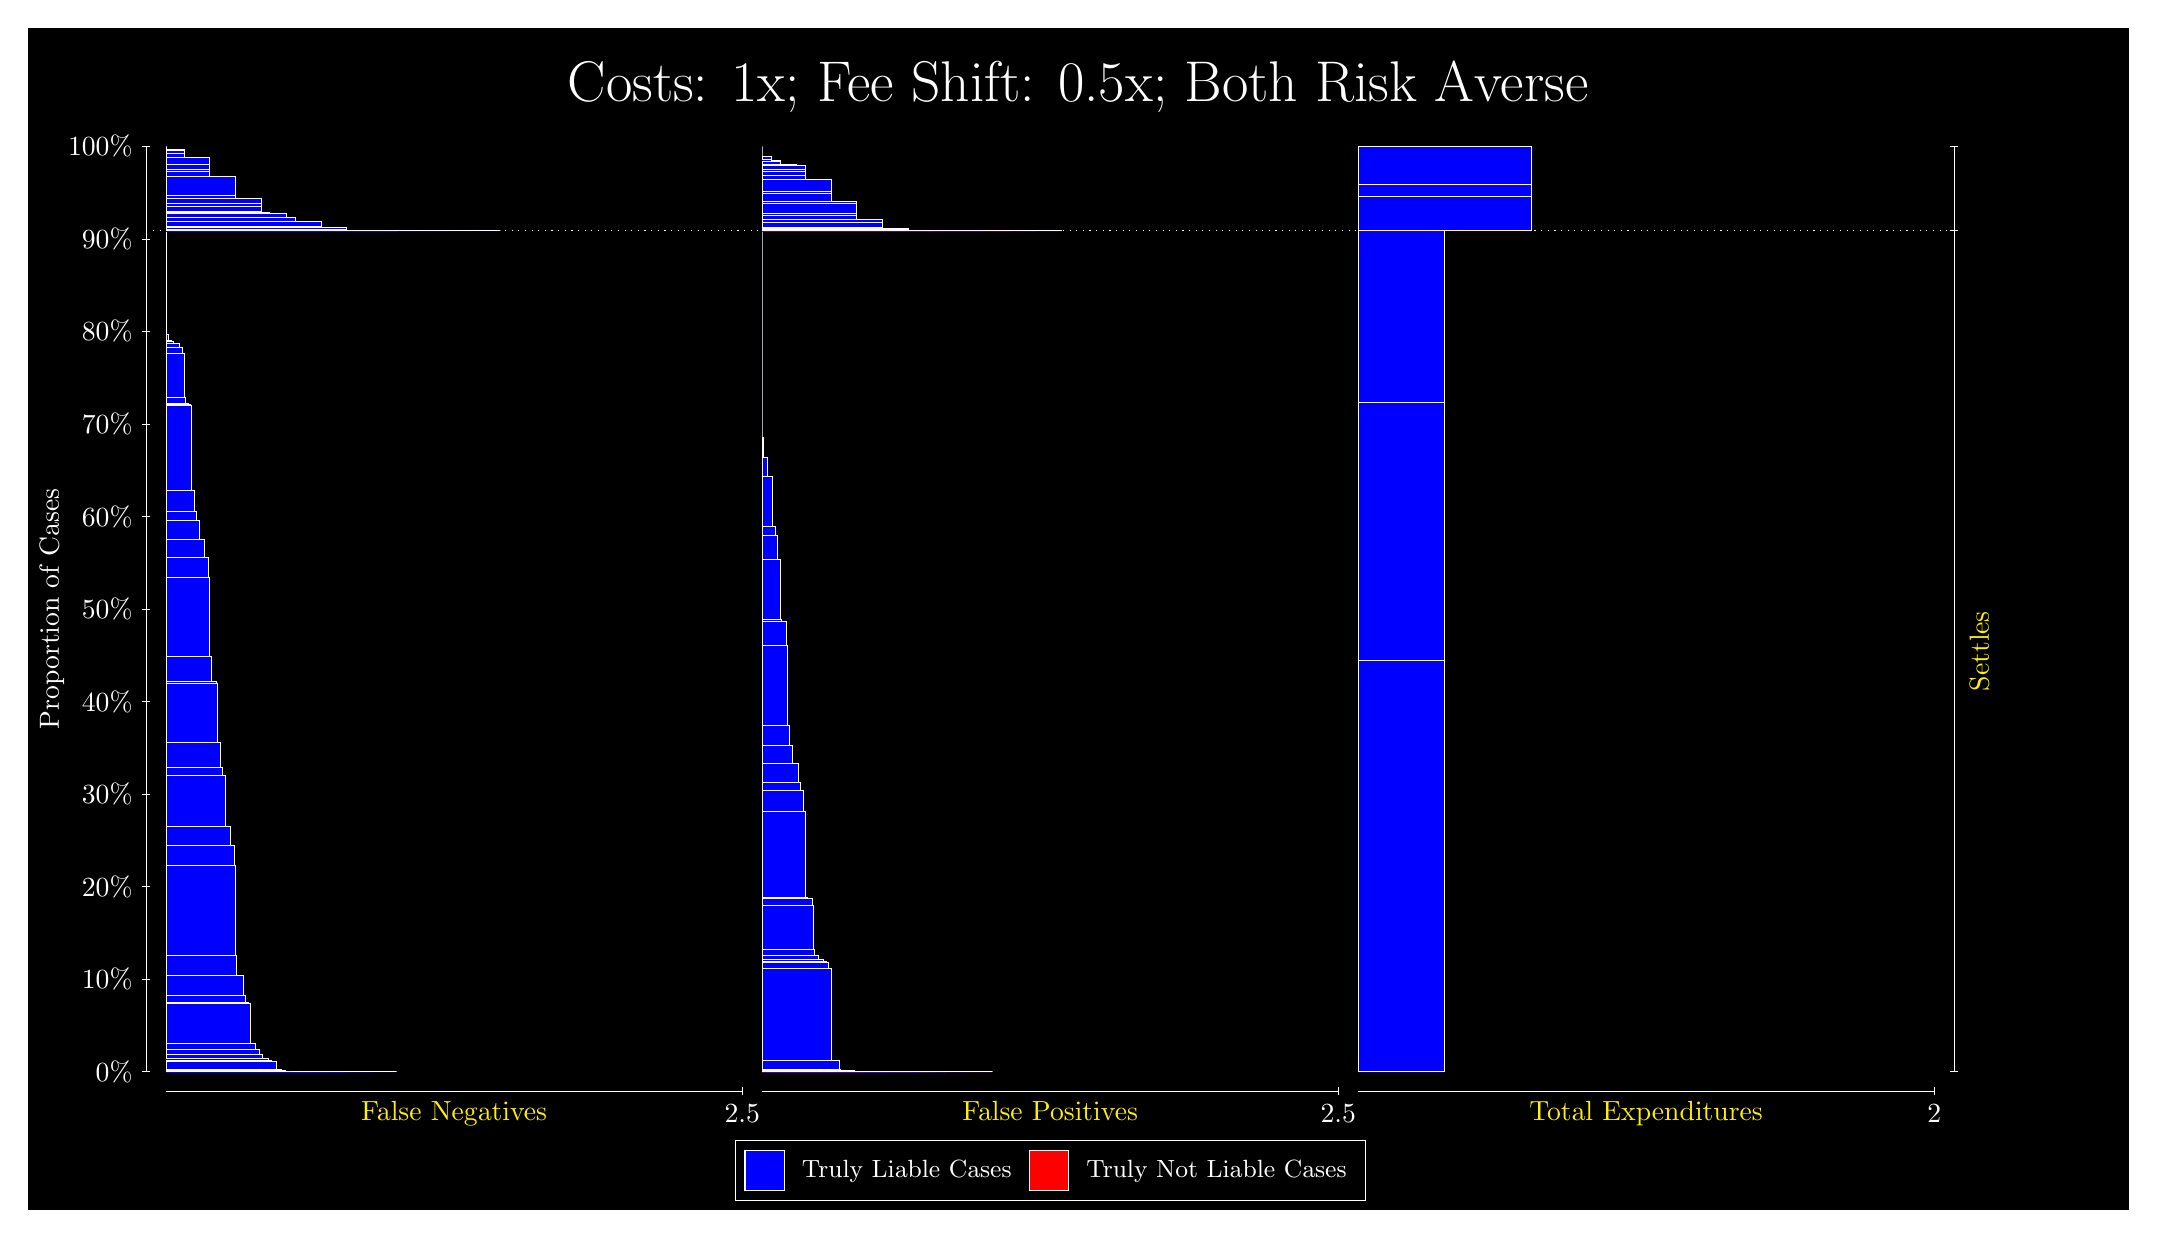
\begin{tikzpicture}
\draw[fill=black] (0,0) rectangle (26.667,15);
\draw[text=white] (0,13.5) rectangle (26.667,15) node[midway] {\huge Costs: 1x; Fee Shift: 0.5x; Both Risk Averse};
\draw[white, very thin] (1.5,1.75) -- (1.5,13.5);
\node[rotate=90, text=white, anchor=center] at (0.3, 7.625) {Proportion of Cases};
\draw[white, very thin] (1.45,1.75) -- (1.55,1.75);
\node[text=white, anchor=east] at (1.45, 1.75) {0\%};
\draw[white, very thin] (1.45,2.925) -- (1.55,2.925);
\node[text=white, anchor=east] at (1.45, 2.925) {10\%};
\draw[white, very thin] (1.45,4.1) -- (1.55,4.1);
\node[text=white, anchor=east] at (1.45, 4.1) {20\%};
\draw[white, very thin] (1.45,5.275) -- (1.55,5.275);
\node[text=white, anchor=east] at (1.45, 5.275) {30\%};
\draw[white, very thin] (1.45,6.45) -- (1.55,6.45);
\node[text=white, anchor=east] at (1.45, 6.45) {40\%};
\draw[white, very thin] (1.45,7.625) -- (1.55,7.625);
\node[text=white, anchor=east] at (1.45, 7.625) {50\%};
\draw[white, very thin] (1.45,8.8) -- (1.55,8.8);
\node[text=white, anchor=east] at (1.45, 8.8) {60\%};
\draw[white, very thin] (1.45,9.975) -- (1.55,9.975);
\node[text=white, anchor=east] at (1.45, 9.975) {70\%};
\draw[white, very thin] (1.45,11.15) -- (1.55,11.15);
\node[text=white, anchor=east] at (1.45, 11.15) {80\%};
\draw[white, very thin] (1.45,12.325) -- (1.55,12.325);
\node[text=white, anchor=east] at (1.45, 12.325) {90\%};
\draw[white, very thin] (1.45,13.5) -- (1.55,13.5);
\node[text=white, anchor=east] at (1.45, 13.5) {100\%};

\draw[white, very thin] (24.457,1.75) -- (24.457,13.5);
\draw[white, very thin] (24.407,1.75) -- (24.507,1.75);
\node[anchor=west] at (24.407, 1.75) {};
\draw[white, very thin] (24.407,12.428) -- (24.507,12.428);
\node[anchor=west] at (24.407, 12.428) {};
\draw[white, very thin] (24.407,13.5) -- (24.507,13.5);
\node[anchor=west] at (24.407, 13.5) {};

\draw[white, very thin, fill=blue] (1.75,1.75) rectangle (4.6775,1.75);
\draw[white, very thin, fill=blue] (1.75,1.75) rectangle (4.3848,1.75);
\draw[white, very thin, fill=blue] (1.75,1.75) rectangle (4.3523,1.75);
\draw[white, very thin, fill=blue] (1.75,1.75) rectangle (4.2384,1.75);
\draw[white, very thin, fill=blue] (1.75,1.75) rectangle (4.092,1.75);
\draw[white, very thin, fill=blue] (1.75,1.75) rectangle (4.0595,1.75);
\draw[white, very thin, fill=blue] (1.75,1.75) rectangle (4.027,1.75);
\draw[white, very thin, fill=blue] (1.75,1.75) rectangle (3.9457,1.75);
\draw[white, very thin, fill=blue] (1.75,1.75) rectangle (3.9131,1.75);
\draw[white, very thin, fill=blue] (1.75,1.75) rectangle (3.7993,1.7501);
\draw[white, very thin, fill=blue] (1.75,1.7501) rectangle (3.7668,1.7501);
\draw[white, very thin, fill=blue] (1.75,1.7501) rectangle (3.7342,1.7501);
\draw[white, very thin, fill=blue] (1.75,1.7501) rectangle (3.7017,1.7501);
\draw[white, very thin, fill=blue] (1.75,1.7501) rectangle (3.6529,1.7501);
\draw[white, very thin, fill=blue] (1.75,1.7501) rectangle (3.6204,1.7501);
\draw[white, very thin, fill=blue] (1.75,1.7501) rectangle (3.5878,1.7502);
\draw[white, very thin, fill=blue] (1.75,1.7502) rectangle (3.474,1.7562);
\draw[white, very thin, fill=blue] (1.75,1.7562) rectangle (3.4415,1.7562);
\draw[white, very thin, fill=blue] (1.75,1.7562) rectangle (3.4089,1.7562);
\draw[white, very thin, fill=blue] (1.75,1.7562) rectangle (3.3764,1.7567);
\draw[white, very thin, fill=blue] (1.75,1.7567) rectangle (3.3602,1.7567);
\draw[white, very thin, fill=blue] (1.75,1.7567) rectangle (3.3276,1.7567);
\draw[white, very thin, fill=blue] (1.75,1.7567) rectangle (3.2951,1.7589);
\draw[white, very thin, fill=blue] (1.75,1.7589) rectangle (3.2626,1.7639);
\draw[white, very thin, fill=blue] (1.75,1.7639) rectangle (3.2138,1.7744);
\draw[white, very thin, fill=blue] (1.75,1.7744) rectangle (3.1487,1.8853);
\draw[white, very thin, fill=blue] (1.75,1.8853) rectangle (3.1162,1.8857);
\draw[white, very thin, fill=blue] (1.75,1.8857) rectangle (3.0837,1.8905);
\draw[white, very thin, fill=blue] (1.75,1.8905) rectangle (3.0511,1.9147);
\draw[white, very thin, fill=blue] (1.75,1.9147) rectangle (3.0349,1.915);
\draw[white, very thin, fill=blue] (1.75,1.915) rectangle (3.0023,1.9151);
\draw[white, very thin, fill=blue] (1.75,1.9151) rectangle (2.9698,1.964);
\draw[white, very thin, fill=blue] (1.75,1.964) rectangle (2.9373,2.032);
\draw[white, very thin, fill=blue] (1.75,2.032) rectangle (2.8885,2.1098);
\draw[white, very thin, fill=blue] (1.75,2.1098) rectangle (2.8234,2.613);
\draw[white, very thin, fill=blue] (1.75,2.613) rectangle (2.7909,2.6302);
\draw[white, very thin, fill=blue] (1.75,2.6302) rectangle (2.7584,2.7178);
\draw[white, very thin, fill=blue] (1.75,2.7178) rectangle (2.7258,2.9684);
\draw[white, very thin, fill=blue] (1.75,2.9684) rectangle (2.7096,2.9732);
\draw[white, very thin, fill=blue] (1.75,2.9732) rectangle (2.6771,2.9755);
\draw[white, very thin, fill=blue] (1.75,2.9755) rectangle (2.6445,3.2216);
\draw[white, very thin, fill=blue] (1.75,3.2216) rectangle (2.6283,4.3756);
\draw[white, very thin, fill=blue] (1.75,4.3756) rectangle (2.612,4.624);
\draw[white, very thin, fill=blue] (1.75,4.624) rectangle (2.5632,4.8705);
\draw[white, very thin, fill=blue] (1.75,4.8705) rectangle (2.4982,5.5064);
\draw[white, very thin, fill=blue] (1.75,5.5064) rectangle (2.4656,5.6151);
\draw[white, very thin, fill=blue] (1.75,5.6151) rectangle (2.4331,5.9263);
\draw[white, very thin, fill=blue] (1.75,5.9263) rectangle (2.4006,6.6821);
\draw[white, very thin, fill=blue] (1.75,6.6821) rectangle (2.3843,6.704);
\draw[white, very thin, fill=blue] (1.75,6.704) rectangle (2.3518,6.7093);
\draw[white, very thin, fill=blue] (1.75,6.7093) rectangle (2.3192,7.0176);
\draw[white, very thin, fill=blue] (1.75,7.0176) rectangle (2.303,8.0304);
\draw[white, very thin, fill=blue] (1.75,8.0304) rectangle (2.2867,8.2809);
\draw[white, very thin, fill=blue] (1.75,8.2809) rectangle (2.2379,8.5073);
\draw[white, very thin, fill=blue] (1.75,8.5073) rectangle (2.1729,8.7507);
\draw[white, very thin, fill=blue] (1.75,8.7507) rectangle (2.1403,8.8595);
\draw[white, very thin, fill=blue] (1.75,8.8595) rectangle (2.1078,9.1261);
\draw[white, very thin, fill=blue] (1.75,9.1261) rectangle (2.0753,10.21);
\draw[white, very thin, fill=blue] (1.75,10.21) rectangle (2.059,10.229);
\draw[white, very thin, fill=blue] (1.75,10.229) rectangle (2.0265,10.231);
\draw[white, very thin, fill=blue] (1.75,10.231) rectangle (1.994,10.319);
\draw[white, very thin, fill=blue] (1.75,10.319) rectangle (1.9777,10.877);
\draw[white, very thin, fill=blue] (1.75,10.877) rectangle (1.9614,10.951);
\draw[white, very thin, fill=blue] (1.75,10.951) rectangle (1.9126,11);
\draw[white, very thin, fill=blue] (1.75,11) rectangle (1.8476,11.024);
\draw[white, very thin, fill=blue] (1.75,11.024) rectangle (1.8151,11.042);
\draw[white, very thin, fill=blue] (1.75,11.042) rectangle (1.7825,11.117);
\draw[white, very thin, fill=red] (1.75,11.117) rectangle (1.75,11.117);
\draw[white, very thin, fill=blue] (1.75,11.117) rectangle (1.75,12.428);
\draw[white, very thin, fill=blue] (1.75,12.428) rectangle (5.9949,12.428);
\draw[white, very thin, fill=blue] (1.75,12.428) rectangle (5.6697,12.428);
\draw[white, very thin, fill=blue] (1.75,12.428) rectangle (5.3444,12.428);
\draw[white, very thin, fill=blue] (1.75,12.428) rectangle (5.3444,12.428);
\draw[white, very thin, fill=blue] (1.75,12.428) rectangle (5.0191,12.428);
\draw[white, very thin, fill=blue] (1.75,12.428) rectangle (4.9052,12.428);
\draw[white, very thin, fill=blue] (1.75,12.428) rectangle (4.6938,12.429);
\draw[white, very thin, fill=blue] (1.75,12.429) rectangle (4.58,12.429);
\draw[white, very thin, fill=blue] (1.75,12.429) rectangle (4.58,12.429);
\draw[white, very thin, fill=blue] (1.75,12.429) rectangle (4.3685,12.436);
\draw[white, very thin, fill=blue] (1.75,12.436) rectangle (4.2547,12.436);
\draw[white, very thin, fill=blue] (1.75,12.436) rectangle (4.2547,12.436);
\draw[white, very thin, fill=blue] (1.75,12.436) rectangle (4.0432,12.451);
\draw[white, very thin, fill=blue] (1.75,12.451) rectangle (4.0432,12.472);
\draw[white, very thin, fill=blue] (1.75,12.472) rectangle (3.9294,12.472);
\draw[white, very thin, fill=blue] (1.75,12.472) rectangle (3.718,12.485);
\draw[white, very thin, fill=blue] (1.75,12.485) rectangle (3.718,12.545);
\draw[white, very thin, fill=blue] (1.75,12.545) rectangle (3.6041,12.55);
\draw[white, very thin, fill=blue] (1.75,12.55) rectangle (3.3927,12.604);
\draw[white, very thin, fill=blue] (1.75,12.604) rectangle (3.2788,12.605);
\draw[white, very thin, fill=blue] (1.75,12.605) rectangle (3.2788,12.653);
\draw[white, very thin, fill=blue] (1.75,12.653) rectangle (3.0674,12.665);
\draw[white, very thin, fill=blue] (1.75,12.665) rectangle (2.9535,12.669);
\draw[white, very thin, fill=blue] (1.75,12.669) rectangle (2.9535,12.737);
\draw[white, very thin, fill=blue] (1.75,12.737) rectangle (2.9535,12.772);
\draw[white, very thin, fill=blue] (1.75,12.772) rectangle (2.9535,12.846);
\draw[white, very thin, fill=blue] (1.75,12.846) rectangle (2.7421,12.846);
\draw[white, very thin, fill=blue] (1.75,12.846) rectangle (2.6283,12.875);
\draw[white, very thin, fill=blue] (1.75,12.875) rectangle (2.6283,13.125);
\draw[white, very thin, fill=blue] (1.75,13.125) rectangle (2.4168,13.125);
\draw[white, very thin, fill=blue] (1.75,13.125) rectangle (2.303,13.181);
\draw[white, very thin, fill=blue] (1.75,13.181) rectangle (2.303,13.207);
\draw[white, very thin, fill=blue] (1.75,13.207) rectangle (2.303,13.271);
\draw[white, very thin, fill=blue] (1.75,13.271) rectangle (2.303,13.356);
\draw[white, very thin, fill=blue] (1.75,13.356) rectangle (2.0915,13.356);
\draw[white, very thin, fill=blue] (1.75,13.356) rectangle (1.9777,13.414);
\draw[white, very thin, fill=blue] (1.75,13.414) rectangle (1.9777,13.451);
\draw[white, very thin, fill=blue] (1.75,13.451) rectangle (1.9777,13.467);
\draw[white, very thin, fill=blue] (1.75,13.467) rectangle (1.7663,13.467);
\draw[white, very thin, fill=red] (1.75,13.467) rectangle (1.75,13.467);
\draw[white, very thin, fill=blue] (1.75,13.467) rectangle (1.75,13.5);
\draw[white, very thin, fill=red] (9.3189,1.75) rectangle (12.246,1.75);
\draw[white, very thin, fill=blue] (9.3189,1.75) rectangle (12.246,1.75);
\draw[white, very thin, fill=blue] (9.3189,1.75) rectangle (11.921,1.75);
\draw[white, very thin, fill=red] (9.3189,1.75) rectangle (11.661,1.75);
\draw[white, very thin, fill=blue] (9.3189,1.75) rectangle (11.661,1.75);
\draw[white, very thin, fill=blue] (9.3189,1.75) rectangle (11.596,1.75);
\draw[white, very thin, fill=red] (9.3189,1.75) rectangle (11.515,1.75);
\draw[white, very thin, fill=blue] (9.3189,1.75) rectangle (11.515,1.75);
\draw[white, very thin, fill=blue] (9.3189,1.75) rectangle (11.336,1.75);
\draw[white, very thin, fill=blue] (9.3189,1.75) rectangle (11.271,1.75);
\draw[white, very thin, fill=red] (9.3189,1.75) rectangle (11.222,1.75);
\draw[white, very thin, fill=blue] (9.3189,1.75) rectangle (11.222,1.75);
\draw[white, very thin, fill=blue] (9.3189,1.75) rectangle (11.189,1.75);
\draw[white, very thin, fill=red] (9.3189,1.75) rectangle (11.075,1.75);
\draw[white, very thin, fill=blue] (9.3189,1.75) rectangle (11.075,1.75);
\draw[white, very thin, fill=blue] (9.3189,1.75) rectangle (11.01,1.75);
\draw[white, very thin, fill=blue] (9.3189,1.75) rectangle (10.945,1.75);
\draw[white, very thin, fill=red] (9.3189,1.75) rectangle (10.929,1.75);
\draw[white, very thin, fill=blue] (9.3189,1.75) rectangle (10.929,1.75);
\draw[white, very thin, fill=blue] (9.3189,1.75) rectangle (10.896,1.75);
\draw[white, very thin, fill=blue] (9.3189,1.75) rectangle (10.864,1.75);
\draw[white, very thin, fill=red] (9.3189,1.75) rectangle (10.783,1.75);
\draw[white, very thin, fill=blue] (9.3189,1.75) rectangle (10.783,1.75);
\draw[white, very thin, fill=blue] (9.3189,1.75) rectangle (10.75,1.7501);
\draw[white, very thin, fill=blue] (9.3189,1.7501) rectangle (10.685,1.7501);
\draw[white, very thin, fill=red] (9.3189,1.7501) rectangle (10.636,1.7501);
\draw[white, very thin, fill=blue] (9.3189,1.7501) rectangle (10.636,1.7505);
\draw[white, very thin, fill=blue] (9.3189,1.7505) rectangle (10.62,1.7557);
\draw[white, very thin, fill=blue] (9.3189,1.7557) rectangle (10.604,1.7558);
\draw[white, very thin, fill=blue] (9.3189,1.7558) rectangle (10.571,1.7558);
\draw[white, very thin, fill=blue] (9.3189,1.7558) rectangle (10.539,1.7558);
\draw[white, very thin, fill=red] (9.3189,1.7558) rectangle (10.49,1.7558);
\draw[white, very thin, fill=blue] (9.3189,1.7558) rectangle (10.49,1.766);
\draw[white, very thin, fill=blue] (9.3189,1.766) rectangle (10.457,1.7665);
\draw[white, very thin, fill=blue] (9.3189,1.7665) rectangle (10.425,1.767);
\draw[white, very thin, fill=blue] (9.3189,1.767) rectangle (10.36,1.7692);
\draw[white, very thin, fill=blue] (9.3189,1.7692) rectangle (10.311,1.7769);
\draw[white, very thin, fill=blue] (9.3189,1.7769) rectangle (10.295,1.8887);
\draw[white, very thin, fill=blue] (9.3189,1.8887) rectangle (10.278,1.8935);
\draw[white, very thin, fill=blue] (9.3189,1.8935) rectangle (10.246,1.8937);
\draw[white, very thin, fill=blue] (9.3189,1.8937) rectangle (10.213,1.8965);
\draw[white, very thin, fill=red] (9.3189,1.8965) rectangle (10.197,1.8965);
\draw[white, very thin, fill=blue] (9.3189,1.8965) rectangle (10.197,3.0605);
\draw[white, very thin, fill=blue] (9.3189,3.0605) rectangle (10.165,3.1363);
\draw[white, very thin, fill=blue] (9.3189,3.1363) rectangle (10.132,3.1537);
\draw[white, very thin, fill=blue] (9.3189,3.1537) rectangle (10.1,3.1779);
\draw[white, very thin, fill=blue] (9.3189,3.1779) rectangle (10.034,3.2269);
\draw[white, very thin, fill=blue] (9.3189,3.2269) rectangle (9.9857,3.3006);
\draw[white, very thin, fill=blue] (9.3189,3.3006) rectangle (9.9694,3.8592);
\draw[white, very thin, fill=blue] (9.3189,3.8592) rectangle (9.9532,3.9469);
\draw[white, very thin, fill=blue] (9.3189,3.9469) rectangle (9.9206,3.9491);
\draw[white, very thin, fill=blue] (9.3189,3.9491) rectangle (9.8881,3.9681);
\draw[white, very thin, fill=blue] (9.3189,3.9681) rectangle (9.8718,5.0517);
\draw[white, very thin, fill=blue] (9.3189,5.0517) rectangle (9.8393,5.3183);
\draw[white, very thin, fill=blue] (9.3189,5.3183) rectangle (9.8068,5.4271);
\draw[white, very thin, fill=blue] (9.3189,5.4271) rectangle (9.7743,5.6705);
\draw[white, very thin, fill=blue] (9.3189,5.6705) rectangle (9.7092,5.8969);
\draw[white, very thin, fill=blue] (9.3189,5.8969) rectangle (9.6604,6.1474);
\draw[white, very thin, fill=blue] (9.3189,6.1474) rectangle (9.6442,7.1602);
\draw[white, very thin, fill=blue] (9.3189,7.1602) rectangle (9.6279,7.4686);
\draw[white, very thin, fill=blue] (9.3189,7.4686) rectangle (9.5954,7.4738);
\draw[white, very thin, fill=blue] (9.3189,7.4738) rectangle (9.5628,7.4958);
\draw[white, very thin, fill=blue] (9.3189,7.4958) rectangle (9.5466,8.2515);
\draw[white, very thin, fill=blue] (9.3189,8.2515) rectangle (9.514,8.5627);
\draw[white, very thin, fill=blue] (9.3189,8.5627) rectangle (9.4815,8.6714);
\draw[white, very thin, fill=blue] (9.3189,8.6714) rectangle (9.449,9.3073);
\draw[white, very thin, fill=blue] (9.3189,9.3073) rectangle (9.3839,9.5538);
\draw[white, very thin, fill=blue] (9.3189,9.5538) rectangle (9.3351,9.8022);
\draw[white, very thin, fill=blue] (9.3189,9.8022) rectangle (9.3189,12.428);
\draw[white, very thin, fill=red] (9.3189,12.428) rectangle (13.125,12.428);
\draw[white, very thin, fill=blue] (9.3189,12.428) rectangle (13.125,12.428);
\draw[white, very thin, fill=red] (9.3189,12.428) rectangle (12.799,12.428);
\draw[white, very thin, fill=blue] (9.3189,12.428) rectangle (12.799,12.428);
\draw[white, very thin, fill=blue] (9.3189,12.428) rectangle (12.474,12.428);
\draw[white, very thin, fill=red] (9.3189,12.428) rectangle (12.474,12.428);
\draw[white, very thin, fill=blue] (9.3189,12.428) rectangle (12.474,12.428);
\draw[white, very thin, fill=blue] (9.3189,12.428) rectangle (12.149,12.428);
\draw[white, very thin, fill=blue] (9.3189,12.428) rectangle (12.149,12.428);
\draw[white, very thin, fill=red] (9.3189,12.428) rectangle (12.149,12.428);
\draw[white, very thin, fill=blue] (9.3189,12.428) rectangle (12.149,12.428);
\draw[white, very thin, fill=red] (9.3189,12.428) rectangle (11.824,12.428);
\draw[white, very thin, fill=blue] (9.3189,12.428) rectangle (11.824,12.428);
\draw[white, very thin, fill=blue] (9.3189,12.428) rectangle (11.824,12.428);
\draw[white, very thin, fill=blue] (9.3189,12.428) rectangle (11.824,12.428);
\draw[white, very thin, fill=red] (9.3189,12.428) rectangle (11.498,12.428);
\draw[white, very thin, fill=blue] (9.3189,12.428) rectangle (11.498,12.432);
\draw[white, very thin, fill=blue] (9.3189,12.432) rectangle (11.498,12.432);
\draw[white, very thin, fill=blue] (9.3189,12.432) rectangle (11.173,12.444);
\draw[white, very thin, fill=red] (9.3189,12.444) rectangle (11.173,12.444);
\draw[white, very thin, fill=blue] (9.3189,12.444) rectangle (11.173,12.461);
\draw[white, very thin, fill=red] (9.3189,12.461) rectangle (11.059,12.461);
\draw[white, very thin, fill=blue] (9.3189,12.461) rectangle (11.059,12.461);
\draw[white, very thin, fill=blue] (9.3189,12.461) rectangle (10.848,12.476);
\draw[white, very thin, fill=blue] (9.3189,12.476) rectangle (10.848,12.541);
\draw[white, very thin, fill=red] (9.3189,12.541) rectangle (10.848,12.541);
\draw[white, very thin, fill=blue] (9.3189,12.541) rectangle (10.848,12.572);
\draw[white, very thin, fill=blue] (9.3189,12.572) rectangle (10.734,12.572);
\draw[white, very thin, fill=red] (9.3189,12.572) rectangle (10.734,12.572);
\draw[white, very thin, fill=blue] (9.3189,12.572) rectangle (10.734,12.572);
\draw[white, very thin, fill=blue] (9.3189,12.572) rectangle (10.522,12.623);
\draw[white, very thin, fill=blue] (9.3189,12.623) rectangle (10.522,12.653);
\draw[white, very thin, fill=blue] (9.3189,12.653) rectangle (10.522,12.775);
\draw[white, very thin, fill=blue] (9.3189,12.775) rectangle (10.522,12.777);
\draw[white, very thin, fill=blue] (9.3189,12.777) rectangle (10.522,12.803);
\draw[white, very thin, fill=red] (9.3189,12.803) rectangle (10.409,12.803);
\draw[white, very thin, fill=blue] (9.3189,12.803) rectangle (10.409,12.803);
\draw[white, very thin, fill=blue] (9.3189,12.803) rectangle (10.409,12.803);
\draw[white, very thin, fill=blue] (9.3189,12.803) rectangle (10.197,12.901);
\draw[white, very thin, fill=blue] (9.3189,12.901) rectangle (10.197,12.93);
\draw[white, very thin, fill=blue] (9.3189,12.93) rectangle (10.197,13.082);
\draw[white, very thin, fill=blue] (9.3189,13.082) rectangle (10.083,13.082);
\draw[white, very thin, fill=red] (9.3189,13.082) rectangle (10.083,13.082);
\draw[white, very thin, fill=blue] (9.3189,13.082) rectangle (10.083,13.082);
\draw[white, very thin, fill=blue] (9.3189,13.082) rectangle (9.8718,13.136);
\draw[white, very thin, fill=blue] (9.3189,13.136) rectangle (9.8718,13.183);
\draw[white, very thin, fill=blue] (9.3189,13.183) rectangle (9.8718,13.207);
\draw[white, very thin, fill=blue] (9.3189,13.207) rectangle (9.8718,13.262);
\draw[white, very thin, fill=blue] (9.3189,13.262) rectangle (9.758,13.264);
\draw[white, very thin, fill=red] (9.3189,13.264) rectangle (9.758,13.264);
\draw[white, very thin, fill=blue] (9.3189,13.264) rectangle (9.758,13.264);
\draw[white, very thin, fill=blue] (9.3189,13.264) rectangle (9.758,13.275);
\draw[white, very thin, fill=blue] (9.3189,13.275) rectangle (9.5466,13.305);
\draw[white, very thin, fill=blue] (9.3189,13.305) rectangle (9.5466,13.323);
\draw[white, very thin, fill=blue] (9.3189,13.323) rectangle (9.4327,13.33);
\draw[white, very thin, fill=blue] (9.3189,13.33) rectangle (9.4327,13.332);
\draw[white, very thin, fill=blue] (9.3189,13.332) rectangle (9.4327,13.378);
\draw[white, very thin, fill=blue] (9.3189,13.378) rectangle (9.3189,13.5);
\draw[white, very thin, fill=red] (16.888,1.75) rectangle (17.986,1.75);
\draw[white, very thin, fill=blue] (16.888,1.75) rectangle (17.986,6.9711);
\draw[white, very thin, fill=red] (16.888,6.9711) rectangle (17.986,6.9711);
\draw[white, very thin, fill=blue] (16.888,6.9711) rectangle (17.986,10.25);
\draw[white, very thin, fill=red] (16.888,10.25) rectangle (17.986,10.25);
\draw[white, very thin, fill=blue] (16.888,10.25) rectangle (17.986,12.428);
\draw[white, very thin, fill=red] (16.888,12.428) rectangle (19.083,12.428);
\draw[white, very thin, fill=blue] (16.888,12.428) rectangle (19.083,12.866);
\draw[white, very thin, fill=red] (16.888,12.866) rectangle (19.083,12.866);
\draw[white, very thin, fill=blue] (16.888,12.866) rectangle (19.083,13.015);
\draw[white, very thin, fill=red] (16.888,13.015) rectangle (19.083,13.015);
\draw[white, very thin, fill=blue] (16.888,13.015) rectangle (19.083,13.5);
\draw[white, dotted] (1.5,12.428) -- (24.457,12.428);
\draw[white, very thin] (1.75,1.5) -- (9.0689,1.5);
\node[text=yellow, anchor=north] at (5.4094, 1.5) {False Negatives};
\draw[white, very thin] (9.0689,1.45) -- (9.0689,1.55);
\node[text=white, anchor=north] at (9.0689, 1.45) {2.5};

\draw[white, very thin] (9.3189,1.5) -- (16.638,1.5);
\node[text=yellow, anchor=north] at (12.978, 1.5) {False Positives};
\draw[white, very thin] (16.638,1.45) -- (16.638,1.55);
\node[text=white, anchor=north] at (16.638, 1.45) {2.5};

\draw[white, very thin] (16.888,1.5) -- (24.207,1.5);
\node[text=yellow, anchor=north] at (20.547, 1.5) {Total Expenditures};
\draw[white, very thin] (24.207,1.45) -- (24.207,1.55);
\node[text=white, anchor=north] at (24.207, 1.45) {2};

\node[text=yellow, centered, rotate=90] at (24.777, 7.0889) {Settles};


\draw (12.978300999999998,1.5) node[draw=none] (baseCoordinate) {};
\begin{scope}[align=center]
        \matrix[scale=0.5, draw=white, below=0.5cm of baseCoordinate, nodes={draw}, column sep=0.1cm]{
            \node[rectangle, draw, minimum width=0.5cm, minimum height=0.5cm, fill=blue] {}; &
            \node[draw=none, font=\small, text=white] (B) {Truly Liable Cases}; &
            \node[rectangle, draw, minimum width=0.5cm, minimum height=0.5cm, fill=red] {}; &
            \node[draw=none, font=\small, text=white] (B) {Truly Not Liable Cases}; \\
            };
\end{scope}

\end{tikzpicture}
\end{document}